% !TEX root = ../main.tex
%
\chapter{Analysis}
\label{sec:4}

\cleanchapterquote{To see a World in a Grain of Sand \\
                   And a Heaven in a Wild Flower \\ 
                   Hold Infinity in the palm of your hand \\
                   And Eternity in an hour}{William Blake}{(Auguries of Innocence)}

In this chapter the details on data sample and the analysis technique used for the search of the \dst
dibaryon and the related antiparticle, will be presented. 
The \dst has been searched in the \dstdecay decay channel, since this is expected to be the
most relevant channel \ -- the expected branching ratio is around 23\% -- \ detectable by the
ALICE apparatus.

From now on, the \dst dibaryon will be identified as \ds as well as \dst, while the deuteron
will be also called $d$.

%
%
\section{Analysis strategy} \label{sec:4.1}

In this section more details are given on the strategy that was decided to use to search the
\dst dibaryon. 
The strategy is to perform a \textbf{blind analysis} for the invariant mass distribution
(\minv) of the \dst \textit{candidates}. A \ds \textit{candidate} is a triplet composed 
by the \ds decay products, or the related antiparticles, in the considered decay channel.
Therefore, a region of interest, where the \ds signal is expected to be, has been defined:
\begin{center}
\textbf{Region of Interest (RoI)}\  $\rightarrow$ \  $(2.280  < $\ \minv$  < 2.480)\ $ \gevcs.
\end{center}
The RoI, will not be considered while studying the selections.
When the selections are satisfactorily optimized the RoI will be \textit{unblinded} and a
background subtraction will be performed to look for the signal.

The idea behind the blind analysis is to optimize the selections and to develop a model
able to describe the background of the measurement without introducing any bias. 

The predicted physics properties of the \dst are summarized in the table \ref{tab:dst_prop}. 
Considering these values, the chosen RoI ensures that the signal \ -- if it exists and it is visible
-- \ is basically in that mass interval.
\begingroup
\renewcommand{\arraystretch}{1.5} % Default value: 1
\begin{table}
\centering
\captionsetup{justification=centering}
\begin{tabular}{lr}
\multicolumn{2}{c}{\textbf{Predicted properties}}      \\
\toprule
Mass				             & 2.380 \ \gevcs 	    \\
$\Gamma$			        	 & 0.070 \ \gevcs 	   	\\
$d\; \pi^{+} \pi^{-}\ $ B.R.	 & 23(2)\ \%		    \\
\midrule
\end{tabular}
\caption{\dst predicted properties.}
\label{tab:dst_prop}
\end{table}
\endgroup

%
%
\section{Data and Monte Carlo sample} \label{sec:4.2}

The analysis presented in this thesis is based on the \pPb collisions at \sctev 
collected in 2016. 

The sample of collected data consists of nearly $5.5\times10^{8}$ minimum bias events.
In order to increase the number of collected events during this data taking period, two
different minimum bias trigger has been adopted.
The first trigger, called \code{CENT}, basically is a minimum bias trigger for the central barrel
detectors. The SDD detector has a greater busy time than other detectors \ -- around three times
than SSD -- \ which limits the rate of collected events. 
In order to increase the rate of collected events, the second trigger, called \code{FAST}, allows
to detect events coming in the SDD busy time by excluding the SDD by the acquisition.
The data flow and triggers management is performed by the ALICE CTP (Section \ref{sec:data_flow}).

In the \textit{off-line} event reconstruction the whole data set analyzed in this work has been
reconstructed excluding the SDD information from the process, in order to made compatible
the data acquired with the two different triggers.

For this analysis two different Monte Carlo data sample has been used.
The first one is a sample of $\sim 5 \times 10^{5}$ \pPb events with injected exotic states
and has been used to study the \dst properties and the reconstruction efficiency of its decay.
The second one is a sample of $\sim 4.6 \times 10^{7}$ \pPb events and has been used to study 
the properties of the background sources of the measurement.

The Monte Carlo data are based the EPOS-LHC generator \cite{epos_lhc} which is an event 
generator for minimum bias hadronic interactions, used for both heavy ion interactions and cosmic 
ray air shower simulations.
Since the EPOS-LHC does not include any (anti-)dibaryon, an \textit{ad-hoc} generator was used to
inject \ds and \dsbar on top of each EPOS-LHC event in the first Monte Carlo sample.
In each generated event are injected ten \dst and ten $\ensuremath{\bar{{d}^{*}}(2380)}$, 
with a homogeneous distribution in transverse momentum \ -- in the $0 \leq \pt \leq 8\;\gevc$ interval
-- \ as well as in the azimuthal angle $\phi$ and in rapidity.
The injected \dst are made decay by the generator through the \dstdecay channel. 

The other possible decay of the \dst have not been considered since are not relevant or not
detectable \ -- because of the presence of neutral particle in the final state -- \ by ALICE.
Since the considered decay occurs through Strong interaction, the decay takes place basically in the 
interaction vertex. Therefore the decay products are generated starting from the interaction vertex
together with the others collision products.

The transport code used for the generation of the detector response \ -- as described
in section \ref{sec:} -- \ is GEANT? 
The data taking conditions are accounted in the MC by reproducing the configuration of the different 
detectors in the runs used for the analysis.

\subsection{Monte Carlo validation} \label{sec:4.2.1}

As mentioned above, the EPOS-LHC event generator does not include the \dst dibaryon, therefore it has
been injected on top of \pPb collision. 
The first thing done in this thesis is the validation of the injection process through
the analysis of the resulting events.
This validation ensure that the injected dibaryonic states have the correct physics properties
expected for the \dst.

This validation has been done checking the shape of the invariant mass distribution of \dst decay 
products, taking the generated tracks. Only tracks from a true \dst and belonging to the same 
mother has been considered, in order to avoid background. 

\begin{figure}
    \centering
    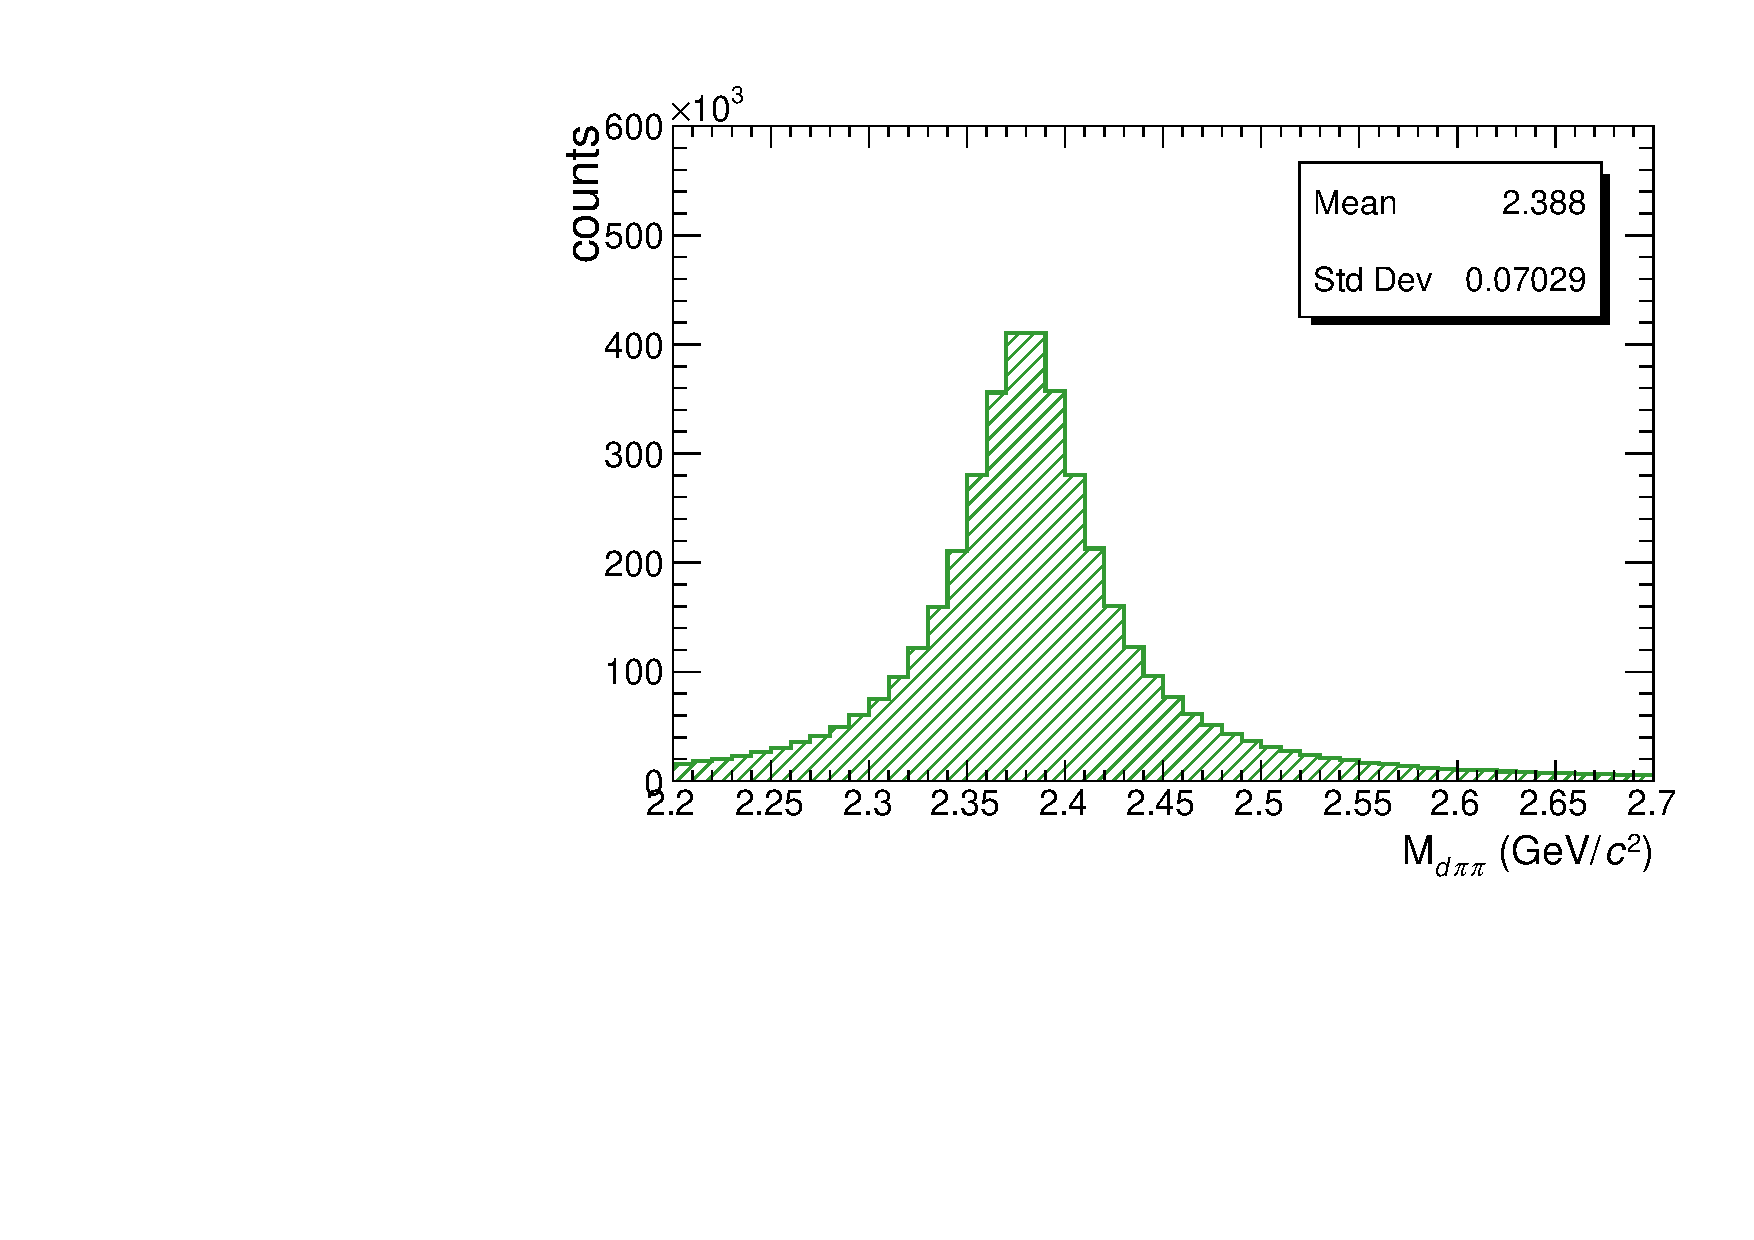
\includegraphics[width=0.6\textwidth]{gfx/valid}
	\caption{Invariant mass distribution of the \dst decay product, obtained using the generated tracks. The distribution shows the correct shape. The mean and the \textit{rms} of the distribution are compatible with the predicted properties of the \dst.}
	\label{fig:valid}
\end{figure}

The signal observed by the WASA-at-COSY collaboration, as discussed in section \ref{sec:wasa}, has
mass of 2380 \mevcs and a width of $\sim$ 70 \mevcs. Therefore, Figure \ref{fig:valid} shows that the
injected signal has the correct features of the \dst.

The momentum spectrum of the pions and deuterons originating from the \ds decay has been checked.
This spectra are reported in Figure \ref{fig:momentum_spec}. 

%
%
\section{Event and track selection} \label{sec:4.2}

In this analysis, the events are analyzed with the \code{CODEX} framework\footnote{The \code{CODEX} 
framework is part of the \code{AliPhysics} software (Section \ref{sec:anal_frame}) and it is 
specifically developed in order to provide analysis tools for the ALICE analysis related to nuclei
production.} that allows to select events with certain features and to store them in a compressed
format.
Such compressed data can be stored and analyzed on local machines, providing an easier and faster 
analysis chain.

Using the \code{CODEX} framework the event and track selection takes part in two different stages.
In the first stage the \code{CODEX} analyze the considered data sample on the WLCG (Section 
\ref{sec:offline}) filtering and storing interesting events in a compressed format. 
Basically, it works as an \textit{off-line} trigger.
In the second stage the filtered data are analyzed on local machines and further track
selections are applied.
In the following sections more details on the event and track selection are provided.

%
\subsection{Event selection: \code{CODEX} filtering}

In the \code{CODEX} filtering the event selection it is done in two steps.
In the first step events are selected using standard ALICE requirements for \pPb events: 
a pile-up rejection exclude events with more than one primary vertex and
a selection based on some features of the primary vertex guarantees the goodness of the
reconstructed vertex.
This last selection, basically reject events for which the vertex reconstructed with full tracks
differs to much from the vertex determined with the SPD only.
More details on the two vertexing processes are given in Section \ref{sec:vertexing}.
The selections applied to the primary vertex in this step are summarized in Table \ref{tab:cod_sel1}.

\begingroup
\renewcommand{\arraystretch}{1.5} % Default value: 1
\begin{table}[hb]
\centering
\begin{tabular}{lr}
\multicolumn{2}{c}{\textbf{Event selection in \code{CODEX}}}        \\
\toprule
$\mid \textit{z} \mid\ $ primary vertex            & $<$ 10 cm      \\
\textit{z}$_{SPD}$ vertex resolution               & $<$ 0.25 cm    \\
$\mid \textit{z}_{SPD} - \textit{z}_{Track} \mid$  & $<$ 0.5 cm	    \\
\midrule
\end{tabular}
\caption{This early selections made in the first step of the \code{CODEX} process ensure a good reconstruction of the primary vertex.}
\label{tab:cod_sel1}
\end{table}
\endgroup

In the second step a track and particle identification selection with loose cuts is performed.
The concept is to store locally only events with a \textit{(anti-)deuteron candidate}, since without
the (anti-)deuteron the \dst decay can't be reconstructed.
The rate of expected (anti-)deuterons in \pPb inelastic collisions is approximately $10^{-4}$,
therefore with this selection it is possible to reduce the number of stored events from at least four
order of magnitude, making the data sample manageable on local machines.

Following the $n\sigma\ $ technique described in \ref{sec:PID}, a track with 
$n\sigma_{TPC} < 5$ and $n\sigma_{TOF} < 10$ for tracks with $\pt > 1.5\; \gevc$,
respect to the deuteron mass hypothesis is considered a \textit{(anti-)deuteron candidate}.
Only events with at least one \textit{(anti-)deuteron candidate} are stored.

%
\subsection{Track selection}

In the second stage the filtered data are processed on local machines, in order to define
the best possible track selections.
Having locally the whole data set of interesting events allows to process the data very 
quickly and therefore to study and to test further track selections easily.
In the following the final selections, established after many attempts, will presented.

Since \dstdecay is a Strong decay only tracks coming from the primary vertex are 
considered in this analysis. Therefore a selection on the DCA \ -- defined in Section
\ref{sec:vertexing} -- \ has been applied. 
The other selections are related to track parameter which describe, somehow, the goodness of the
reconstruction process of the track. 
In order to use only the geometrical region where the ALICE experiment is able to perform a full
tracking and to provide the best possible PID information, only tracks in the pseudorapidity 
region $|\eta| < 0.9 $ are selected. This requirements is mainly related to the TPC acceptance,
since it is the main used detector. 
Moreover, to guarantee a track momentum resolution better than 5\% and a TPC \dedx resolution of
6\%, the selected tracks are required to have at least 70 clusters in the TPC.
Then the selected tracks are required to overcome successfully the ITS and the TPC refit process
\ -- described in Section \ref{sec:tarcking}.
In addition, the $\chi^{2}$ per TPC clusters is computed in the track fitting procedure and is
required to be less than 4, while the \textit{Golden $\chi^{2}$} \ -- defined as blah blah blah -- 
\ is required to be less than 36.
Finally, further selection is applied on the \code{kKink} parameter in order to reject
particles coming from beam line interactions.

\begingroup
\renewcommand{\arraystretch}{1.5} % Default value: 1
\begin{table}
\centering
\begin{tabular}{cc}
\multicolumn{2}{c}{\textbf{Track selection criteria}} \\
\toprule
Variable                            &   Selection        \\
\midrule
$\mid \eta \mid$  				    &	$\leq$ 0.9	     \\
TPC clusters	                    &	$>$ 70		     \\
$\chi^{2}$ per TPC clusters		    &	$<$ 4		     \\
Golden $\chi^{2}$                   &   $<$ 36           \\
TPC refit					        &	\code{true}		 \\
ITS refit						    &	\code{true}		 \\
Kink daughters			       		& 	rejected		 \\
DCA$_{xy}$					        &	$<$ $(0.0105+0.0350) / \ensuremath{\pt}^{1.1}$  cm \\
DCA$_{z}$					        &	$<$ 2 cm    	 \\
\midrule
\end{tabular}
\caption{Summary of the track selections applied in the analyses of the 2016 data sample.}
\label{table:tselection}
\end{table}
\endgroup

The aforementioned track selection criteria are applied to all the analyses presented in this
thesis and are summarized in Table \ref{tab:tracksel}

%
% 
\section{Reconstruction of the \ds} \label{sec:ds_candidate}

After the event and track selection there is nothing left but to determine the (\dsbar)\ds candidates.
And this is done by selecting the daughter tracks of the two charged pions decay:
\begin{equation}
    \dstdecay.
\end{equation}
Therefore a (\dsbar)\ds candidate is a triplet of tracks identified as (anti-)deuteron, \pip and
\pim.

The determination of the particle species of the track is performed with a track-by-track
selection on the $n\sigma$ variable as described in Section \ref{sec:PID}. One of the main
challenges in this analysis is to be able to have a good identification of the deuteron in the 
momentum range in which the \ds production is expected to be more abundant. But, at the same time,
it is essential to have a high purity of the pions and deuterons samples.
Therefore the choice of the detectors which are to be used for the PID is not trivial and should
be investigated.

\begin{figure}
    \centering
    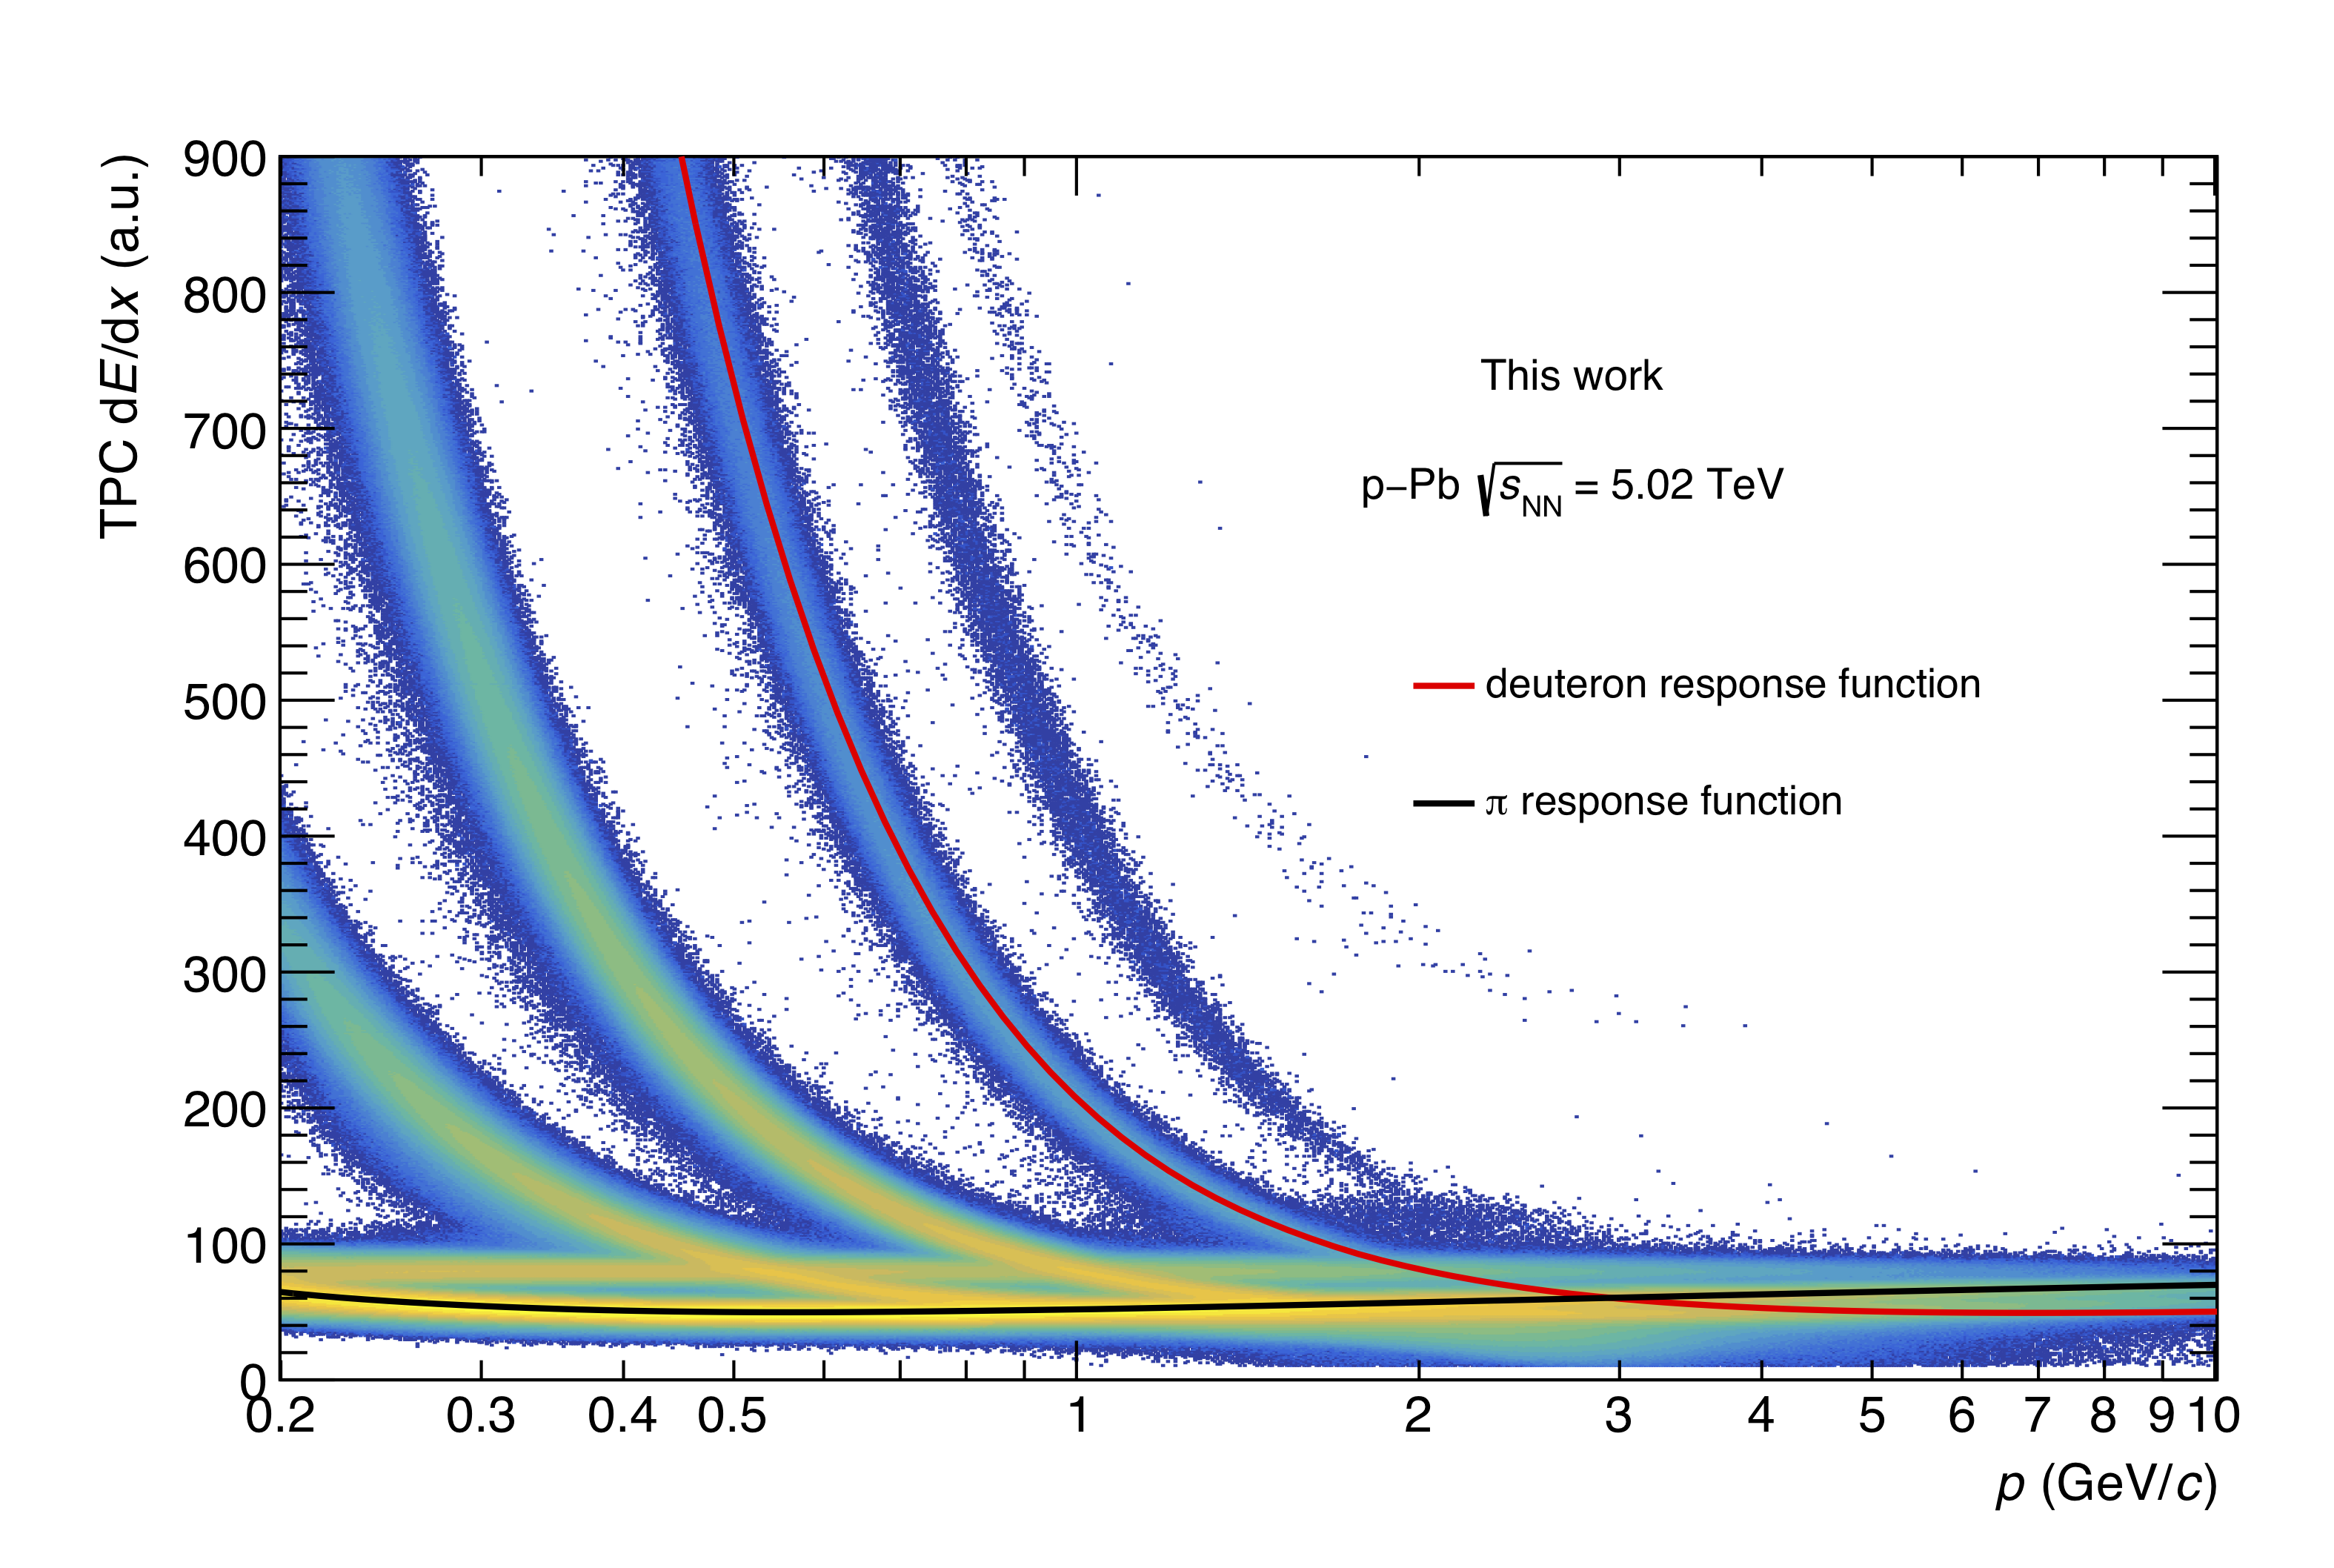
\includegraphics[width=0.8\textwidth]{gfx/pid_tpc}
	\caption{Specific energy loss in the TPC active volume as a function of the particle rigidity in \pPb collisions for the 2016 data sample. The solid lines represent the expected TPC response for pion (black) and deuteron (red).}
	\label{fig:tpc_pid_this}
\end{figure}

A clear identification of the (anti-)deuteron using the TPC information only, is possible for
tracks up to $p \sim 1.2\; \gevc$ due to the finite resolution on the specific energy loss measured by
the TPC and the contamination from electrons and positrons (Figure \ref{fig:tpc_pid_this}).
Using the TOF detector is possible to have an unambiguous identification of the (anti-)deuteron for
tracks up to $p \sim 2\; \gevc$ and still good identification for tracks up to $p \sim 6\; \gevc$.
Therefore combining TPC and TOF information can improve PID for particle with enough momentum to 
reach the TOF.

Otherwise the identification of the pion in the TPC is limited by the contamination from kaons and
protons an can be performed for tracks up to $p \sim 1\; \gevc$. Using the TOF for pions
identification can improve the purity of the sample, but at the same time can dramatically reduce the
reconstruction efficiency of the \ds decay, since the pions produced by the \ds are expected to be at
low momentum as shown in Figure \ref{fig:momentum_spec}.

In order to determine which PID configuration ensures the best performances in the reconstruction
of the \ds decay 3 PID configurations have been studied. The choice of the configuration used
for the search of the \ds will be dictated by the performances in the reconstruction of the decay
and in the signal/background ratio.

\paragraph{PID configurations:}
\begin{itemize}
\item \textbf{TPC:} PID performed only with TPC for both pions and deuterons.
\item \textbf{TPC+TOF:} PID performed with TPC and TOF for both pions and deuterons.
\item \textbf{TPC+TOF$_{deuteron}$:} pions identified with TPC only and deuterons
identified with both TPC and TOF.
\end{itemize}

For each configuration, the same selections are applied on the $n\sigma$ variable as reported in
Table \ref{tab:pid_config}.

\begingroup
\renewcommand{\arraystretch}{1.5} % Default value: 1
\begin{table}
\centering
\begin{tabular}{ccc}
    & \multicolumn{2}{c}{\textbf{PID selections}}  \\%& \multicolumn{2}{c}{\textbf{Selections for TOF}}\\
\toprule
Species & Selection for TPC & Selection for TOF   \\
\hline
$\pi$ & $\mid n \sigma_{TPC}\mid\; \leq 3.$  & $\mid n \sigma_{TOF}\mid\; \leq 3.$ \\

$d$   & $\mid n \sigma_{TPC}\mid\; \leq 3.$  & $\mid n \sigma_{TOF}\mid\; \leq 3.$ \\
\midrule
\end{tabular}
\caption{Selection applied for the identification of candidate $\pi$ and $d$ using the TPC and TOF detectors.}
\label{tab:pid_config}
\end{table}
\endgroup

%
%
\section{Spectrum shape estimation} \label{sec:spectrum}

As reported in Section \ref{sec:4.2}, in the Monte Carlo productions the \dst was injected with flat
transverse momentum spectrum in the $0 \leq \pt \leq 8\;\gevc$ interval. 
This study is performed in order to have a more realistic spectrum both for the \ds and for the decay 
products.


Assuming the same \pt spectrum of the deuteron for the \ds, it is possible to obtain the \ds 
transverse momentum spectrum with a rejection sampling. The deuteron spectrum in \pPb collisions is
described by the Blast Wave (BW) distribution, which is based on the phenomenological model for
hadronic matter production in heavy ion collisions, published in \cite{blastwave}.
The distribution is written as:
\begin{equation}
    \frac{1}{\pt} \frac{d\,N}{d\,\pt} \propto \int_{0}^{R} r\,dr\,m_{\mathrm{T}} I_{0}
    \left( \frac{\pt \sinh\rho}{T_{kin}} \right) K_{1} \left( \frac{m_{\mathrm{T}} \cosh\rho}
    {T_{kin}} \right),
\end{equation}
where the parameter $\rho$ contains the dependence on the velocity profile, since it is expressed
as:
\begin{equation}
    \rho = \tanh^{-1} \left[ \left( \frac{r}{R} \right)^{n} \beta_{s} \right]
\end{equation}
In the previous equations $m_{\mathrm{T}} = \sqrt{\pt^{2} + m^{2}}$ is the transverse mass,
$I_{0}$ and $K_{1}$ the modified Bessel functions, $r$ is the radial distance on the transverse plane,
$T_{kin}$ is the kinetic freeze-out temperature, $\beta_{s}$  the surface velocity of the expanding 
medium and $n$ is the exponent of the velocity profile.
\begingroup
\renewcommand{\arraystretch}{1.5} % Default value: 1
\begin{table}
\centering
\begin{tabular}{lc}
\multicolumn{2}{c}{\textbf{Blast wave parameters}} \\
\toprule
Parameter       &   Value            \\
\midrule
$m$			    &	1.8756 \gevcs    \\
$n$             &   1.97208          \\
$T_{kin}$       &   0.128583         \\
$\beta_{s}$     &   0.710369         \\
\midrule
\end{tabular}
\caption{Values of the parameters of the Blast Wave distribution used, in this analysis, as a basis fo the rejection method implemented to obtain a realistic spectrum for the \ds in the Monte Carlo.}
\label{tab:bw_param}
\end{table}
\endgroup
The parameters values, used in this analysis and summarized in Table \ref{tab:bw_param}
were obtained by fitting the measured deuterons spectrum with the BW distribution in previous
analysis.

The rejection sampling has been applied to the \ds generated in the Monte Carlo, obtaining a 
plausible \pt spectrum for the \ds and its decay product. In Figure \ref{fig:bw_spectrum} the
resulting \pt spectrum is shown both before (blue line) and after (magenta line) the reconstruction
process.

\begin{figure}
    \centering
    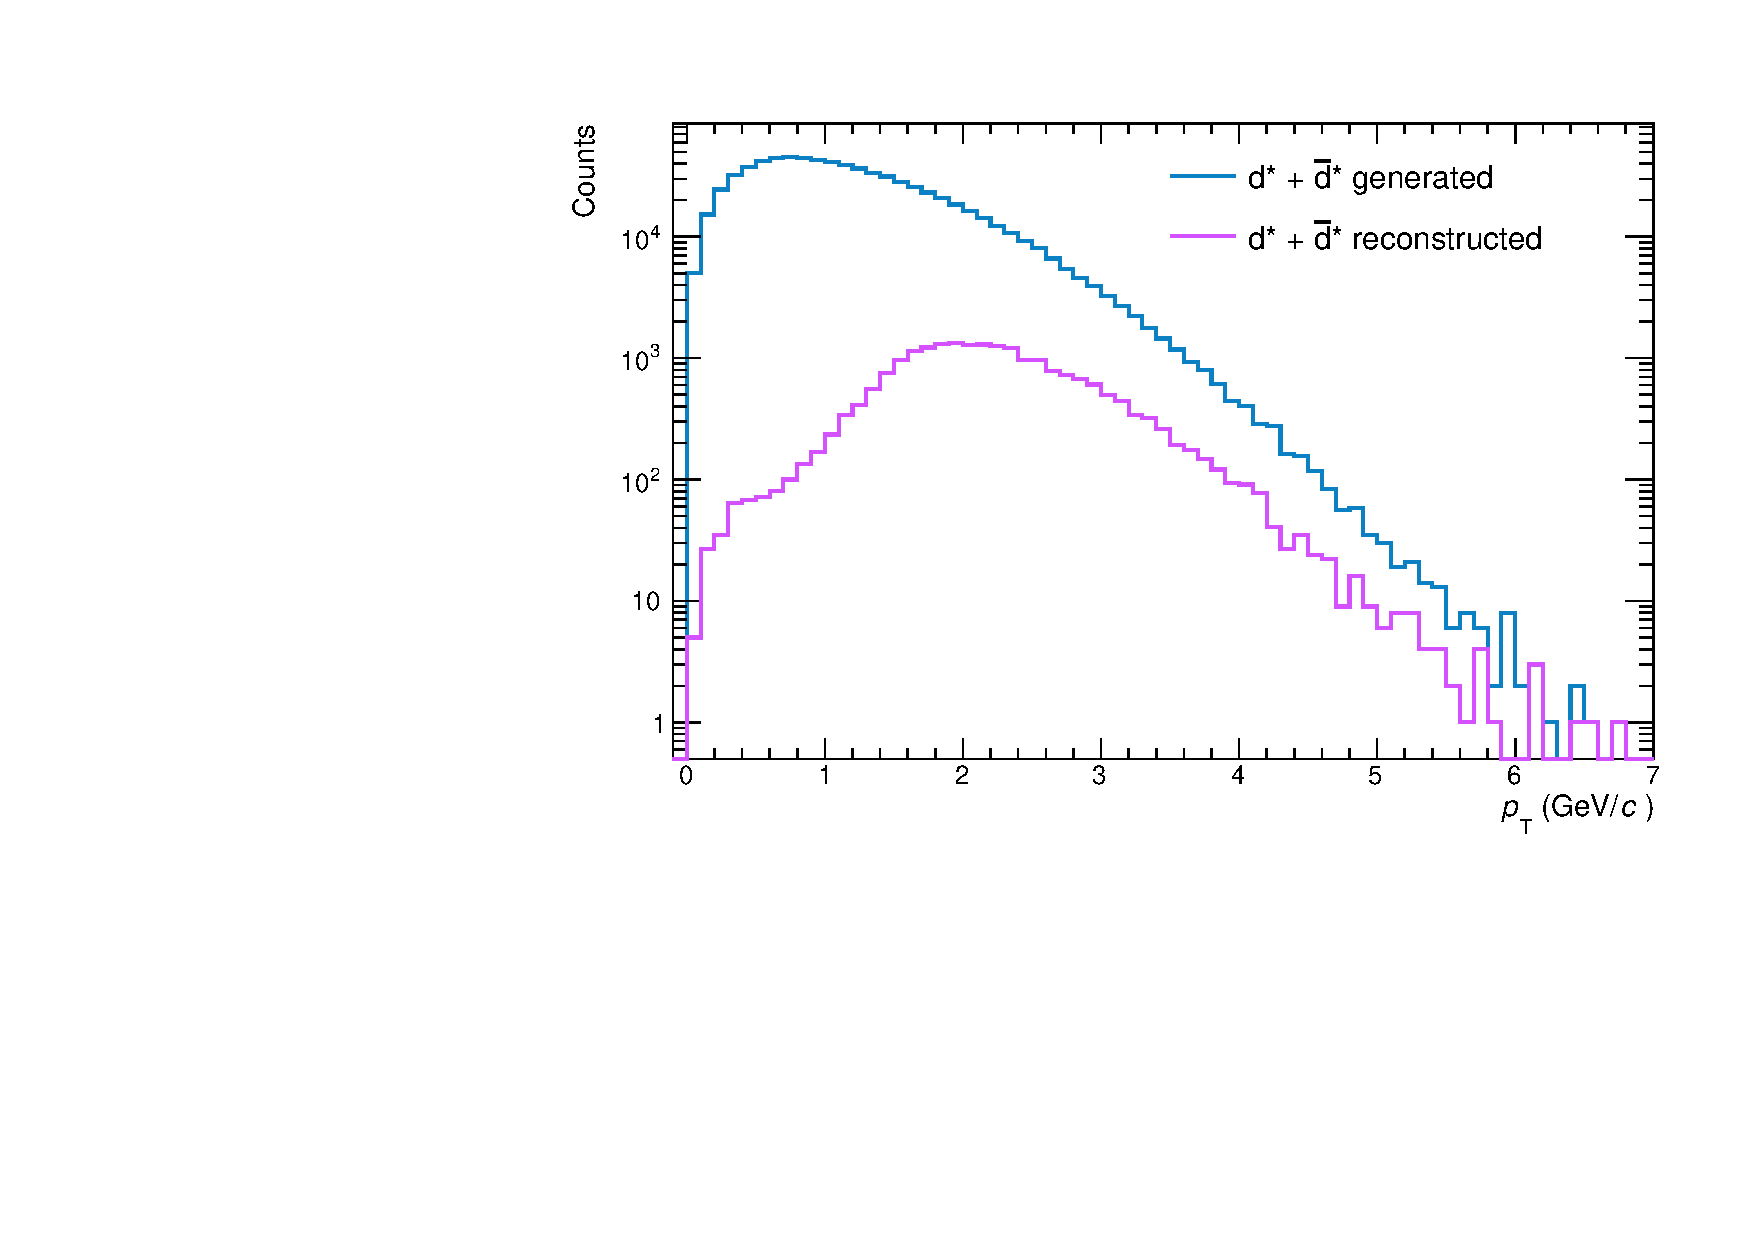
\includegraphics[width=0.5\textwidth]{gfx/genrecBW}
	\caption{Spectrum for both generated (blue line) and reconstructed (magenta line) \ds obtained with Blast Wave rejection sampling.}
	\label{fig:bw_spectrum}
\end{figure}

%
%
\section{Reconstruction efficiency of the \ds decay} \label{sec:eff}

One of the fundamental steps of the analysis presented in this thesis is to evaluate if the
\dstdecay is detectable by the ALICE apparatus, considering reconstruction efficiency and acceptance
of the ALICE detectors. 

Furthermore, if the decay is visible, the measured raw yields are biased by inefficiencies in the
ALICE detectors.
For instance, the active area of the experiment is not hermetic by design or, sometimes, parts of the
detectors might be switched off during some data taking periods due to technical problems, reducing
the efficiency.
The acceptance, instead, is only related to the geometric coverage of the detectors.

It is possible to correct for the finite efficiency and acceptance using a MC simulation where the
full geometry and the real data taking conditions are reproduced. The MC production used for this
analysis has been described in Section \ref{sec:4.2}. 
The number of particles crossing the detectors and their kinematics observables are known when using
the MC simulation and the efficiency$\times$acceptance can be computed as:
\begin{equation}
    Efficiency \times Acceptance\ (\pt) = \frac{\mathrm{N}_{\textit{rec}}(\pt)}
    {\mathrm{N}_{\textit{gen}}(\pt)},
\end{equation}
where $\mathrm{N}_{\textit{gen}}$ is the number (\dsbar)\ds generated in the azimuthal region
$0 \leq \phi < 2\pi$ and in the $|y| < 0.5$, while $\mathrm{N}_{\textit{rec}}$ is the number of 
(\dsbar)\ds for which the decay products satisfies the selection criteria described in Section
\ref{sec:}. % mettere la 



% The aim af this stage is to select tracks which are \textit{candidate daughters} of
% the \dst decay. Therefore, to be accepted, a track must be a good track \ -- in terms 
% of the selections described in the following -- \ and must be identified as a charged 
% pion or an (anti-)deuteron.
